\documentclass{standalone}
\usepackage{tikz}
\usepackage{circuitikz}
\usetikzlibrary{positioning}

\begin{document}
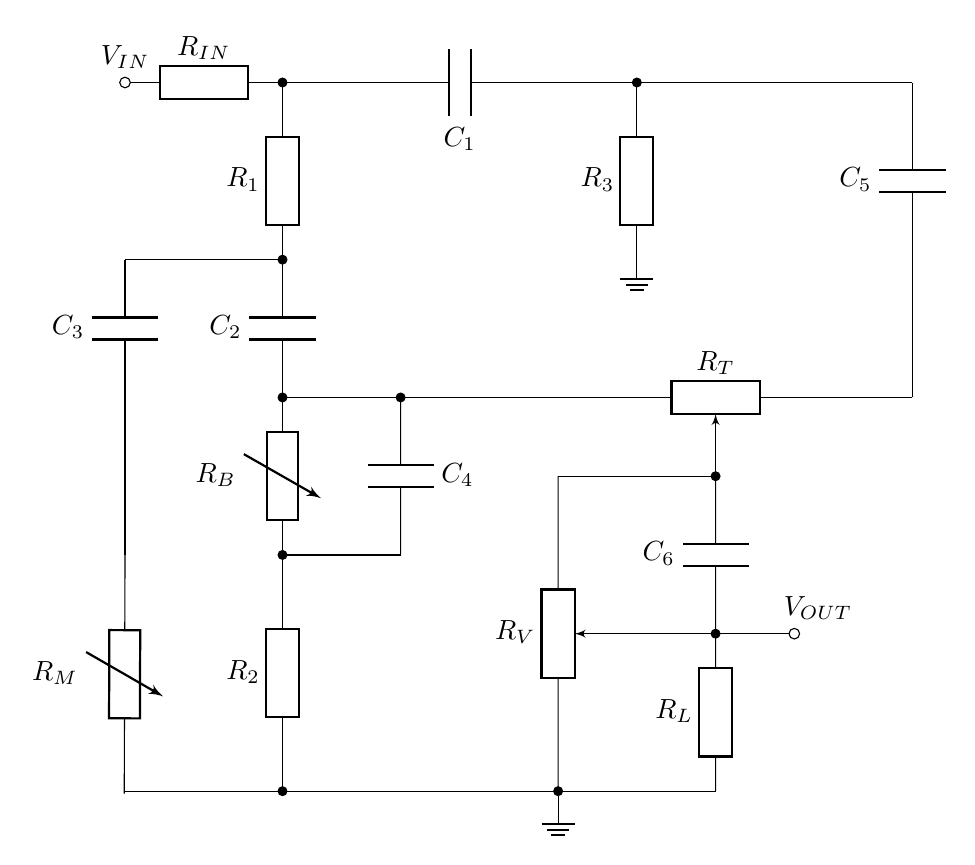
\begin{tikzpicture}
	% Instances/Symbols:
	\draw (3.5, 10) to[european resistor, l=$R_{IN}$] (5.5, 10);
	\draw (5.5, 9.75) to[european resistor, l_=$R_1$] (5.5, 7.75);	
	\draw (5.5, 4) to[european resistor, l_=$R_2$] (5.5, 1);	
	\draw (10, 10) to[european resistor, l_=$R_3$] (10, 7.5);
	\draw (11, 3) to[european resistor, l_=$R_L$] (11, 1);

	\draw (5.5, 10) to[capacitor, l_=$C_1$] (10, 10);
	\draw (5.5, 7.75) to[capacitor, l_=$C_2$] (5.5, 6);
	\draw (3.5, 7.75) to[capacitor, l_=$C_3$] (3.5, 6);
	\draw (7, 6) to[capacitor, l=$C_4$] (7, 4);
	\draw (13.5, 10) to[capacitor, l_=$C_5$] (13.5, 7.5);
	\draw (11, 5) to[capacitor, l_=$C_6$] (11, 3);
	
	\draw (5.5, 6) to[variable european resistor, l_=$R_B$] (5.5, 4);
	\draw (3.5, 4) to[variable european resistor, l_=$R_M$] (3.49, 0.97);
	\draw (13.5, 6) to[european potentiometer, l_=$R_T$] (8.5, 6);
	\draw (9, 5) to[european potentiometer, l_=$R_V$] (9, 1);

	% Lines:
	\draw (11, 3) -- (9.5, 3);
	\draw (11, 3) -- (12, 3);
	\draw (13.5, 7) -- (13.5, 7.5);
	\draw (10, 10) -- (13.5, 10);
	\draw (3.5, 4) -- (3.5, 6);
	\draw (3.5, 7.75) -- (5.5, 7.75);
	\draw (5.5, 9.75) -- (5.5, 10);
	\draw (7, 4) -- (5.5, 4);
	\draw (5.5, 6) -- (7, 6);
	\draw (9, 5) -| (11, 5);
	\draw (11, 5.44) -- (11, 5);
	\draw (13.5, 7) -- (13.5, 6);
	\draw (8.5, 6) -- (7, 6);
	\draw (3.5, 1) -- (11, 1);	

	\node[tlground] at (10, 7.5) {};
	\node[ground] at (9, 1) {};

	% Nodes:
	\node[circ] at (5.5, 10) {};
	\node[circ] at (10, 10) {};	
	\node[circ] at (5.5, 1) {};
	\node[circ] at (5.5, 4) {};
	\node[circ] at (5.5, 6) {};
	\node[circ] at (5.5, 7.75) {};
	\node[circ] at (7, 6) {};
	\node[circ] at (9, 1) {};
	\node[circ] at (11, 5) {};
	\node[circ] at (11, 3) {};
	\node[ocirc, scale=1.2] at (12, 3) {};
	\node[ocirc, scale=1.2] at (3.5, 10) {};

	% Labels
	\node[above=0.05cm of {3.5, 10}] {$V_{IN}$};
	\node[above=0.05cm of {12.3, 3}] {$V_{OUT}$};

\end{tikzpicture}
\end{document}